%%%%%%%%%%%%%%%%%%%%%%%%%%%%%%%%%%%%%%%%%
% Stylish Article
% LaTeX Template
% Version 2.1 (1/10/15)
%
% This template has been downloaded from:
% http://www.LaTeXTemplates.com
%
% Original author:
% Mathias Legrand (legrand.mathias@gmail.com) 
% With extensive modifications by:
% Vel (vel@latextemplates.com)
%
% License:
% CC BY-NC-SA 3.0 (http://creativecommons.org/licenses/by-nc-sa/3.0/)
%
%%%%%%%%%%%%%%%%%%%%%%%%%%%%%%%%%%%%%%%%%

%----------------------------------------------------------------------------------------
%	PACKAGES AND OTHER DOCUMENT CONFIGURATIONS
%----------------------------------------------------------------------------------------

\documentclass[fleqn,10pt]{SelfArx} % Document font size and equations flushed left
\usepackage[english]{babel} % Specify a different language here - english by default

\setlength{\columnsep}{0.55cm} % Distance between the two columns of text
\setlength{\fboxrule}{0.75pt} % Width of the border around the abstract

\definecolor{color1}{RGB}{0,0,90} % Color of the article title and sections
\definecolor{color2}{RGB}{0,20,20} % Color of the boxes behind the abstract and headings

\usepackage{hyperref} % Required for hyperlinks
\hypersetup{hidelinks,colorlinks,breaklinks=true,urlcolor=color2,citecolor=color1,linkcolor=color1,bookmarksopen=false,pdftitle={Title},pdfauthor={Author}}

\usepackage[capitalise]{cleveref}
\usepackage{float}
% 
\usepackage[colorinlistoftodos,prependcaption,textsize=small]{todonotes}
%----------------------------------------------------------------------------------------
%	ARTICLE INFORMATION
%----------------------------------------------------------------------------------------

\JournalInfo{ANS report} % Journal information
\Archive{BGP sim} % Additional notes (e.g. copyright, DOI, review/research article)

\PaperTitle{BGP pySim documentation} % Article title

\Authors{Lorenzo Ghiro} % Authors
%\affiliation{\textsuperscript{1}\textit{Department of Biology, University of Examples, London, United Kingdom}} % Author affiliation
%\affiliation{\textsuperscript{2}\textit{Department of Chemistry, University of Examples, London, United Kingdom}} % Author affiliation
%\affiliation{*\textbf{Corresponding author}: john@smith.com} % Corresponding author

\Keywords{} % Keywords - if you don't want any simply remove all the text between the curly brackets
\newcommand{\keywordname}{Keywords} % Defines the keywords heading name

\Abstract{A python simulator has been developed to replicate the exponential path exploration problem described in \cite{fabrikant2011there}. The simulator workflow and kind of events, together with the BGP node logic implemented by the pySim, are described in this document.}

\begin{document}
\flushbottom % Makes all text pages the same height
\maketitle % Print the title and abstract box
%\tableofcontents % Print the contents section
\thispagestyle{empty} % Removes page numbering from the first page

\section{Simulator high-level architecture} 
%\addcontentsline{toc}{section}{Introduction}
The simulator requires:
\begin{enumerate}[noitemsep]
  \item The network topology, described by a graphml file
  \item The output folder
\end{enumerate}

\section{Initialization}
The graphml is parsed to:
\begin{enumerate}[noitemsep]
  \item initialize node objects with their TYPE and prefixes to be exported
  \item setup neighbourhood relationships. This includes peering or customer/provider role assignment and per-neigh default-MRAI assignment
\end{enumerate}

\section{Node implementation}\label{sec:nodeLogic}

\subsection*{Node attributes}
A node has/is described by, and keeps updated the following:
\begin{enumerate}[noitemsep]
  \item nodeID and nodeType
  \item \textbf{neighs}: a dictionry with neighID as keys and \textit{(relation, mrai)} as neighbour attributes
  \item \textbf{exportPrefixes}: a list of prefixes exported by this node
  \item \textbf{RoutingTable}: an object with convenient methods to install routes and to remeber received updates, so to be ready to install backup routes
\end{enumerate}

\subsubsection*{Routing table}
A routing table is a dictionary indexed by known prefixes. For each prefix these info are kept updated:
\begin{enumerate}[noitemsep]
  \item NH and AS-PATH
  \item PREFERENCE, computed according to the \textbf{policy function}\footnote{The policy function comes as a separate py file, to ease extension and multiple versions implementation in the future}
  \item MRAIs: a dictionary indexed by neighbours' ids. For each neigh the time after which is possible to send an update is maintained.
  \item SHARED-FLAG: again a per-neigh indexed dictionary. A flag per neighbour is maintained to remember if an update has been sent or not to this neigh for this prefix. Thanks to these flags and assuming no losses in sending updates over TCP connections, we will see the network "\textit{silent}" at convergence.
  \item adjRIBin: again per-neigh dict. The last update received from the indexed neigh for the given prefix is maintained here
\end{enumerate}

\subsection*{PROCESSING received updates}
When a node receives an update, it schedules its own "state-transition" after a short delay. This delay model the non-zero time required to process an update.
After this delay, the node run a (instantaneous) DECISION-PROCESS, deciding what to do with the received update. This process may trigger the sending of an update.

\subsection*{SENDING updates}
The send-update routine is responsible to disseminate those routes that, compared to the last sent update, are new or have been modified (modified once or multiple time).
The send-update can fail therefore if:
\begin{enumerate}[noitemsep]
  \item the route-to-announce has been already shared with neighbours
  \item the mrai for the announced prefix (with a given neigh), has not expired
\end{enumerate}

\section{Decision Process}

Nodes react to only one kind of event, called: DECISION-PROCESS. The event is scheduled when nodes receive an update or set an mrai.
In the first case, the DECISION-PROCESS starts after a little delay, modelling the non-zero processing time \cite{fabrikant2011there}.
In the 2nd case, the DECISION-PROCESS is triggered when an mrai expires so that, if a node has a route still not shared with neighbour, 
then will send updates. The full decision process is illustrated by \cref{fig:decisionprocess}.

\begin{figure}[ht]
\centering
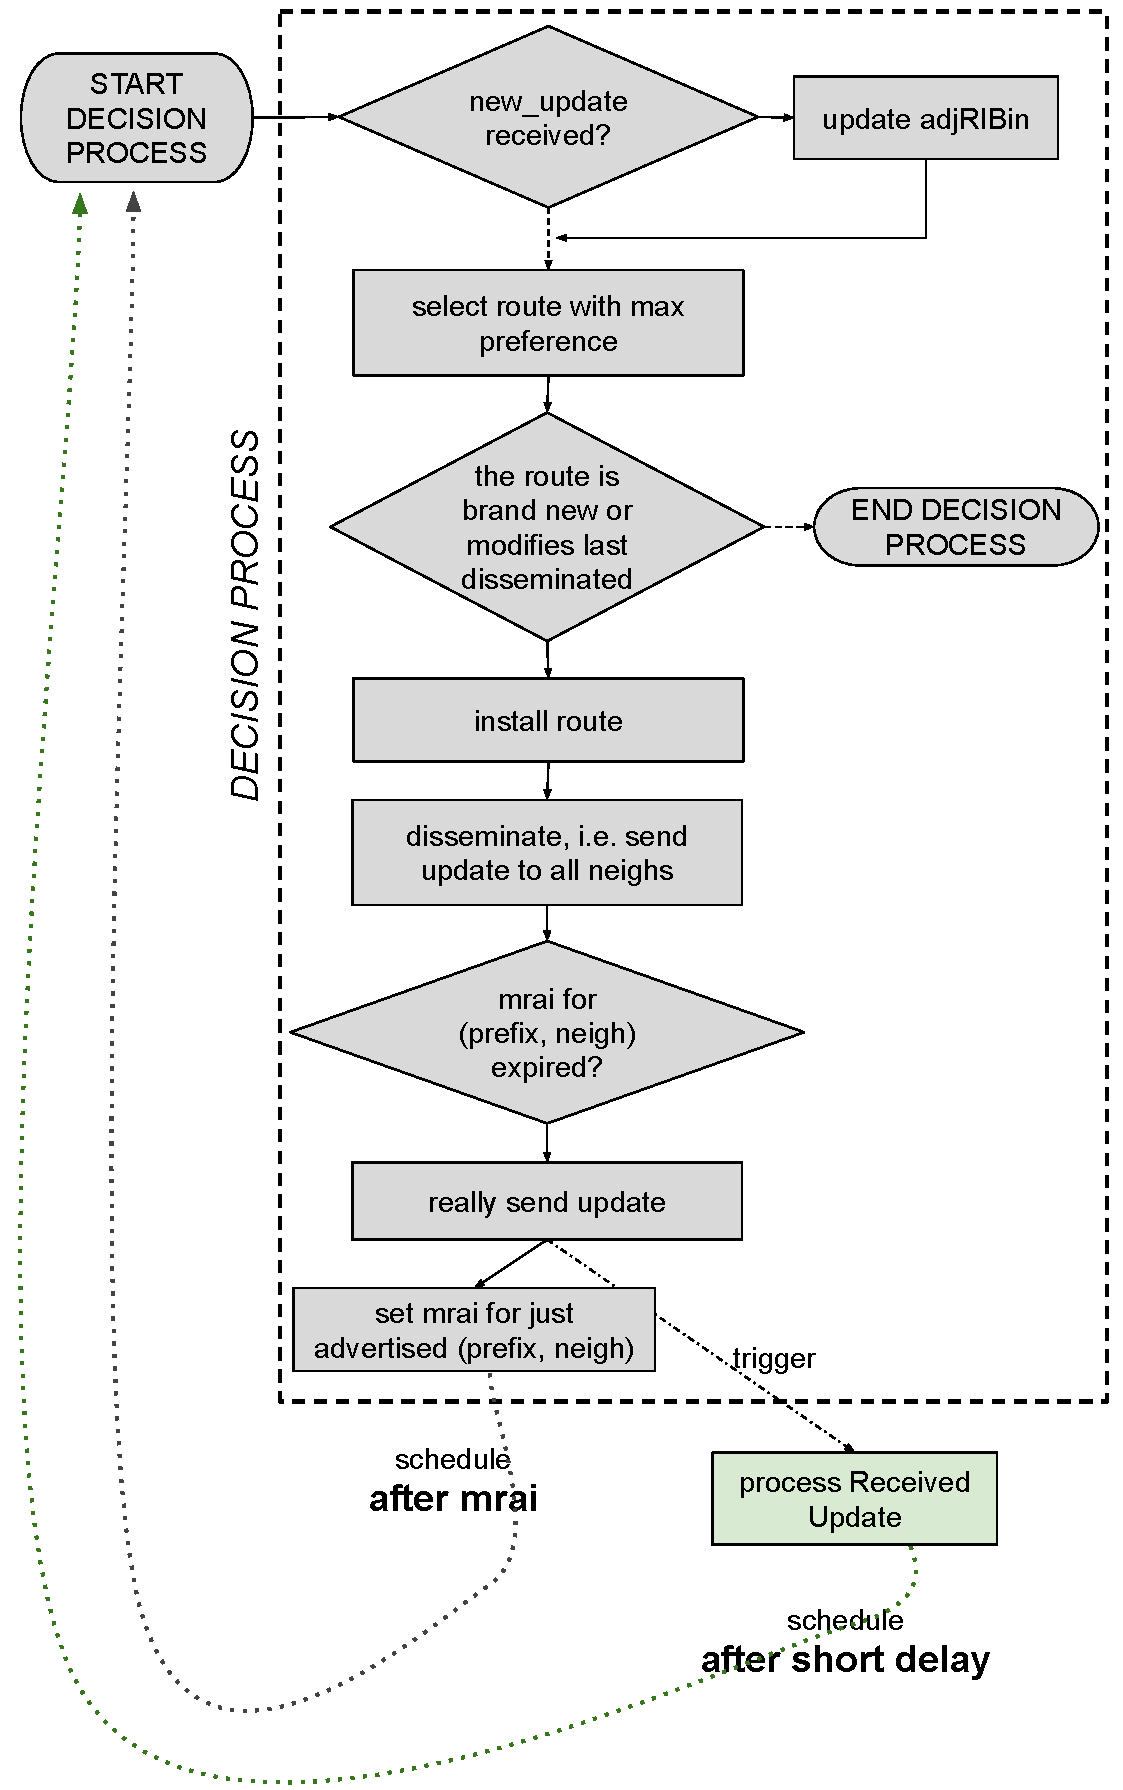
\includegraphics[width=\linewidth]{figures/workflow}
\caption{Decision Process. In grey the main actions of a node, in green the actions triggered for neighbouring node.}
\label{fig:decisionprocess}
\end{figure}

\paragraph{Workflow}
\begin{enumerate}[noitemsep]
  \item Put received updates in the adjRIBin
  \item Phase 1: Compute PREFERENCE applying the policy function to all updates in adjRIBin 
  \item Phase 2: For each destination (in our case just one), select and install the route with higher preference. 
    	If the best\&installed route is related to a new or modified route, then the installing routine sets the 
    	SHARED-FLAG of this route to False (i.e. not shared yet, an advertisement must be sent).
  \item Phase 3 (Dissemination): The node tries to send updates about routes that have been not shared yet. Fails if MRAI is not expired.
  		In case of success, the SHARED-FLAG is reset to True and MRAI is reset as well.
\end{enumerate}

\section{First results}

Based on the usual topology (\cref{})
\begin{figure}[ht]
\centering
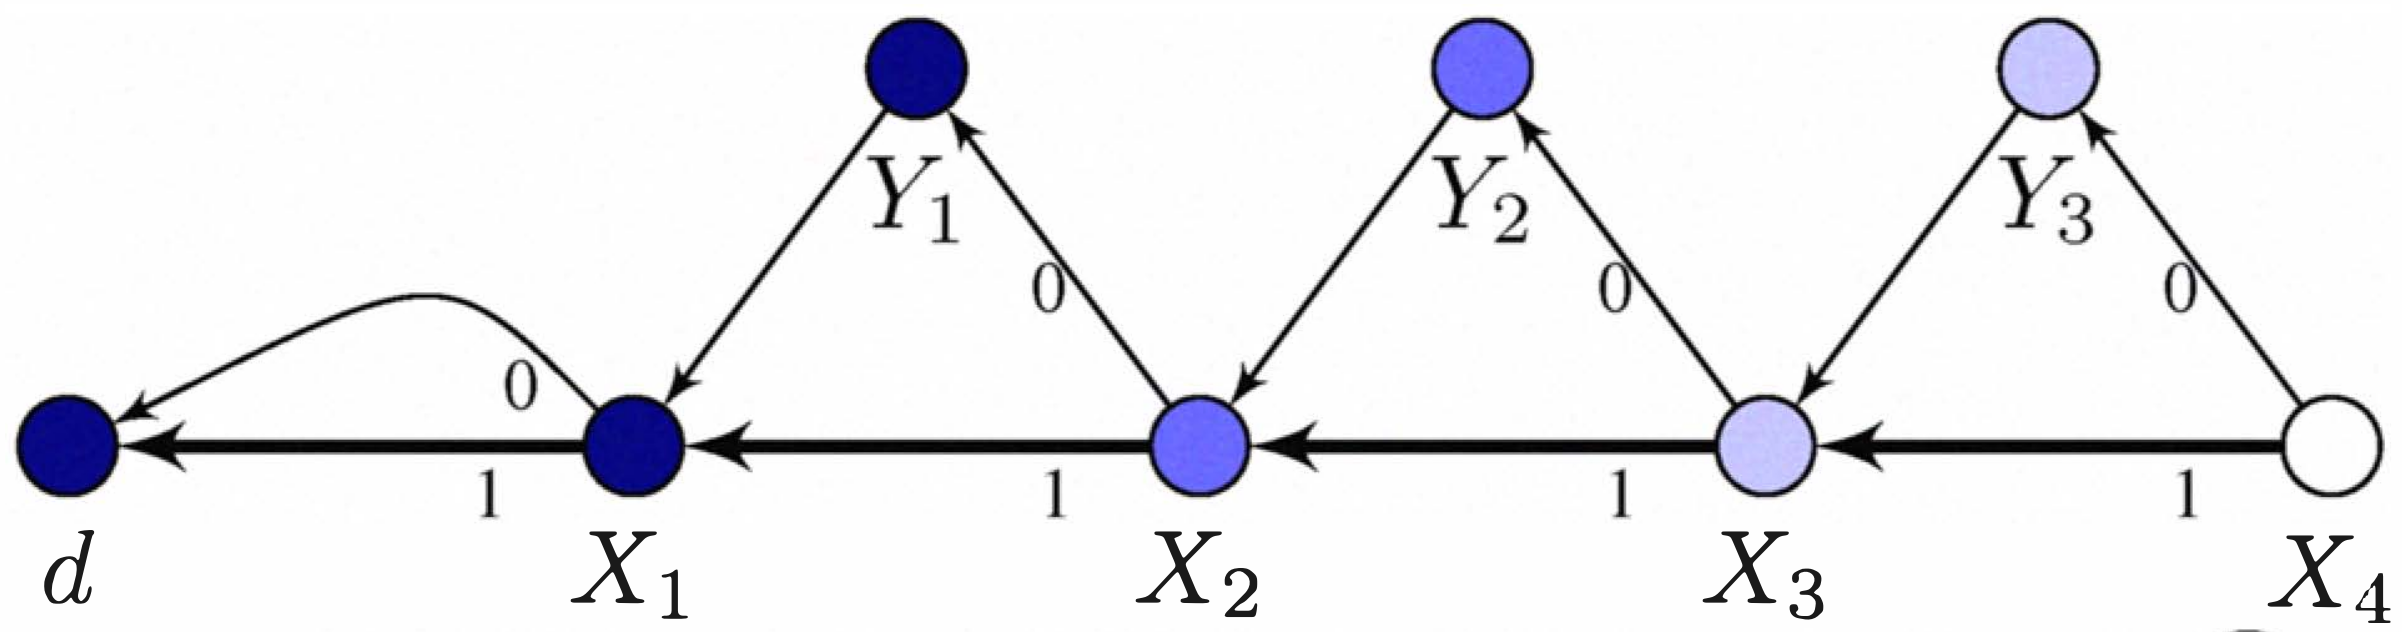
\includegraphics[width=\linewidth]{figures/fabrex.png}
\caption{The usual reference topology}
\label{fig:decisionprocess}
\end{figure}

%----------------------------------------------------------------------------------------
%	REFERENCE LIST
%----------------------------------------------------------------------------------------
\phantomsection
\bibliographystyle{IEEEtran}
\bibliography{sample}

%----------------------------------------------------------------------------------------

\end{document}


%----------------------------------------------------------------------------------------


%\begin{figure*}[ht]\centering % Using \begin{figure*} makes the figure take up the entire width of the page
%\includegraphics[width=\linewidth]{view}
%\caption{Wide Picture}
%\label{fig:view}
%\end{figure*}



%\begin{table}[hbt]
%\caption{Table of Grades}
%\centering
%\begin{tabular}{llr}
%\toprule
%\multicolumn{2}{c}{Name} \\
%\cmidrule(r){1-2}
%First name & Last Name & Grade \\
%\midrule
%John & Doe & $7.5$ \\
%Richard & Miles & $2$ \\
%\bottomrule
%\end{tabular}
%\label{tab:label}
%\end{table}